%\section{Exploração do Dataset}
%
%Numa primeira fase foram criadas funções para explorar o conjunto de dados. \\
%
%A função \textbf{col\_names} retorna-nos uma dataframe com todos os nomes das colunas. A função \textbf{n\_contracts} retorna-nos o número de linhas, ou seja, o número de contratos totais, da base de dados. \\
%
%Foi desenvolvida, também, uma função \textbf{h} que permite ver uma dataframe de forma mais apresentável.\\
%
%\textit{É preciso criar uma função com o código que já tenho para categorizar os contratos de acordo com o tipo de procedimento. Idem para o tipo de contrato.} \\

 

%\begin{table}[H]
%	\centering
%	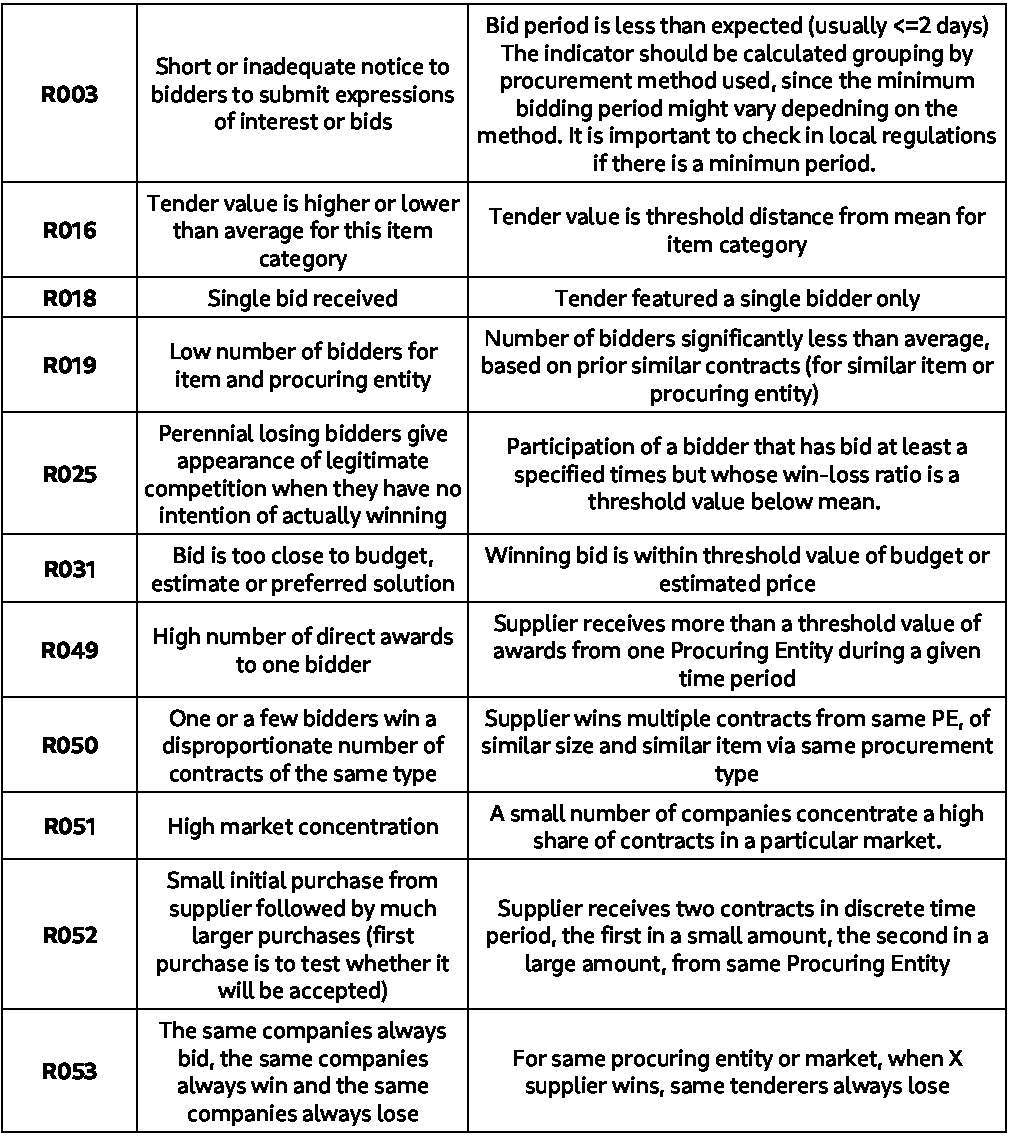
\includegraphics[width= \textwidth]{tabelas/tabela_rf.pdf}
%	\caption{}
%	\label{}
%\end{table}



 

%\section{Funções Auxiliares}
%
%Para a construção das \textit{flags} são necessárias outras funções mais simples. Certas funções irão ter um único propósito e os outputs de certas funções irão ser usados como inputs de outras funções. \\
%
%Para identificar um contrato necessitamos do seu id. Assim, criou-se uma função \textbf{all\_ids} que retorna os ids de todos os contratos da base de dados. Contudo, como não vamos trabalhar com todos os tipos de contratos e procedimentos, é necessário filtrar estes ids.
%Para tal, criaram-se as funções \textbf{ajustes\_dir}, \textbf{consulta\_prev} e \textbf{concurso\_pub} que retornam os ids de todos os ajustes diretos, consultas prévias e concursos públicos, respetivamente. \\
%
%De seguida, filtraram-se os contratos por tipo de procedimento e por CPV. Para isso, criou-se a função \textit{cpv\_direto} que retorna todos os ids de ajustes diretos para serviços de consultoria em IT ( todos os CPV's começados por 72). De seguida, foi feito o mesmo para contratos públicos na função \textit{cpv\_cpub}. De forma a generalizar, criou-se a função \textit{cpv} que retorna todos os ids de contratos de um tipo de procedimento e para um determinado CPV. Tanto o tipo de procedimento como os primeiros 2 algarismos do CPV são parâmetros de entrada da função. \\
%
%
%Para começar, criaram-se duas funções que permitem ver qual é o contrato associado a um determinado id. A função \textit{contrato} tem como input um único id de um contrato ( todas estas funções dizem respeito à tabela \textit{contratos} da DB) e retorna uma dataframe com uma única linha referente ao contrato associado a esse mesmo id. A função \textit{contratos} faz exatamente a mesma coisa mas para um conjunto de id's. \\
%
%Quando as flags estiverem construídas e quisermos ver o anúncio de um contrato suspeito no site do basegov, podemos fazê-lo usando a função \textit{url} que, novamente, tem como parâmetro de entrada o id de um contrato. Esta função pode ter bastante utilidade nos casos que chamam bastante a atenção, como por exemplo, quando se viu um ajuste direto de 3 milhões de euros. \\



\section{Contratação Fechada}

\subsection{RF1 : Verificação dos Preços Contratuais para Ajustes Diretos em Regime Geral}


Como foi apresentado anteriormente na tabela 1.4, os ajustes diretos tem diferentes limites máximos impostos por lei, mediante o tipo de obra/serviço. 
A fim de poder identificar os contratos que não estão em conformidade com o CCP, foi necessário fazer algumas alterações na base de dados. Primeiro, foi necessário classificar o ajuste direto de acordo com o critério. Se os critério for Critério do Valor, os valores máximos permitidos são os que se encontram presentes na tabela 1.4. Se o critério for Critério Material, estamos perante uma situação em que pode ser adotado o ajuste direto independentemente do valor do contrato a celebrar. Assim, a partir da coluna \textit{fundamentacao} da tabela, pode-se verificar qual o artigo do CCP adotado para realizar o ajuste direto. 


\begin{table}[H]
	\centering
	\begin{tabular}{|c|c|c|c|}
		\hline
		\textbf{Critério}                  & \textbf{Artigos}           & \textbf{Tipo de Contrato}           & \textbf{Valor} \\ \hline
		\multirow{3}{*}{Critério do Valor} & \multirow{3}{*}{17º a 22º} & Aquisição de bens móveis e serviços & 20000€         \\ \cline{3-4} 
		&                            & Empreitadas de obras públicas       & 30000 €        \\ \cline{3-4} 
		&                            & Outro tipo de contratos             & 50000 €        \\ \hline
		Critério Material                  & 24º a 27º                  & Qualquer                            & Indefinido     \\ \hline
	\end{tabular}
	\caption{text}
\end{table}

Assim, foi criada uma nova coluna \textit{artigo} que, a partir da coluna \textit{fundamentacao}, guarda apenas o artigo presente - ignora as alíneas. 

\begin{lstlisting}[
	language=SQL,
	showspaces=false,
	showstringspaces=false,
	basicstyle=\ttfamily,
	numbers=left,
	numberstyle=\tiny,
	commentstyle=\color{gray}, frame = single,	autogobble=true,
	postbreak=\mbox{\textcolor{red}{$\hookrightarrow$}\space},
	]
	ALTER TABLE ajustesdiretos
	ADD COLUMN artigo text;
	
	UPDATE ajustesdiretos
	SET artigo = TRIM(SUBSTRING(fundamentacao 
			FROM 1 FOR POSITION('º' IN fundamentacao)));
\end{lstlisting}





De seguida, foi criada uma coluna \textit{criterio}, constituída apenas por duas strings : valor e material. Para um determinado contrato, se o artigo no campo \textit{fundamentacao} pertencer entre o 17º e o 22º, então é-lhe atribuído o critério valor. Caso contrário, o cirtério material. 


\begin{lstlisting}[
	language=SQL,
	showspaces=false,
	showstringspaces=false,
	basicstyle=\ttfamily,
	numbers=left,
	numberstyle=\tiny,
	commentstyle=\color{gray}, frame = single,	autogobble=true,
	postbreak=\mbox{\textcolor{red}{$\hookrightarrow$}\space},
	]
	ALTER TABLE ajustesdiretos
	ADD COLUMN criterio text;
	
	UPDATE ajustesdiretos
	SET criterio = CASE
	WHEN artigo = 'Artigo 17.º' OR artigo = 'Artigo 18.º' 
	OR artigo = 'Artigo 19.º' OR artigo = 'Artigo 20.º' 
	OR artigo = 'Artigo 21.º' OR artigo = 'Artigo 22.º' 
	THEN 'valor'
	
	ELSE 'material' 
	END;
\end{lstlisting}


Assim, é possível identificar todos os contratos que não respeitem os valores apresentados nas tabelas 1.4 e 4.1 através das seguintes \textit{queries} : 

\begin{lstlisting}[
	language=SQL,
	showspaces=false,
	showstringspaces=false,
	basicstyle=\ttfamily,
	numbers=left,
	numberstyle=\tiny,
	commentstyle=\color{gray}, frame = single,	autogobble=true,
	breaklines=true,
	postbreak=\mbox{\textcolor{red}{$\hookrightarrow$}\space},
	]
	SELECT * FROM ajustesdiretos
	WHERE criterio = 'valor' AND tipocontrato = 'Bens e Servicos' AND preco > 20000;
	
	SELECT * FROM ajustesdiretos
	WHERE criterio = 'valor' AND 
	tipocontrato = 'Empreitadas' AND preco > 30000;
\end{lstlisting}




%Esta função tem como input uma dataframe correspondente a todos os ajustes diretos realizados com CPV 72, sendo esta obtida fazendo uso dos funções \textit{contratos} e \textit{cpv} definidas antes, e os ids dos contratos associados aos ajustes diretos. 
%A função vai comparar todos os preços contratuais com o valor de 20.000€ pois é o limite máximo de aquisição de serviços. Esta parte tem de  ser atualizada no futuro. Contudo, a maior parte dos ajustes diretos é Aquisição de Serviços. Se os valores forem superiores a este preço, é ativada uma flag.
%A segunda parte da função verifica se foi feita uma fundamentação para o ajuste direto. Esta vai ser sempre uma alínea qq do CCP. Mas tem de estar preenchida. Se o valor ultrapassar os 20000€ e não estiver fundamentado é claramente comportamento suspeito. Se o contrato só tiver a parte da fundamentação por preencher, pode ser má prática. 








\section{Contratação Aberta}

\subsection{R003 : Análise do Prazo de Apresentação de Propostas}


\Lemma{}
{
	Short or inadequate notice to bidders to submit expressions of interest or bids. Bid period is less than expected (usually <=2 days)
	The indicator should be calculated grouping by procurement method used, since the minimum bidding period might vary depedning on the method.  It is important to check in local regulations if there is a minimun period.  
}


De acordo com o artigo 135.º do CCP, o prazo mínimo para apresentação de propostas num concurso público não pode ser inferior a 6 dias e, no caso de se tratar de um procedimento de formação de um contrato de empreitada de obras públicas, a 14 dias. Assim, foi criada uma coluna adicional, \textit{tipocontrato}, para a criação desta flag a partir da coluna \textbf{contratCtypes}. Sempre que, para um determinado contrato, o tipo de contrato contiver a palavra Empreitada, é atribuída a string \textit{Empreitada} à nova coluna. Caso contrário, é atribuída a string \textit{Bens e Serviços}. De seguida, foi construída uma \textit{query} em PostgreSQL para determinar todos os contratos referentes a concursos públicos que não respeitam estas condições. \\


\begin{lstlisting}[
	language=SQL,
	showspaces=false,
	showstringspaces=false,
	basicstyle=\ttfamily,
	numbers=left,
	numberstyle=\tiny,
	commentstyle=\color{gray}, frame = single,
	autogobble=true,
	breaklines=true,
	postbreak=\mbox{\textcolor{red}{$\hookrightarrow$}\space},
	]
	SELECT concursospublicos."id"
	FROM concursospublicos
	WHERE tipocontrato = 'Empreitadas' AND prazo_execucao < 14;
	
	SELECT concursospublicos."id"
	FROM concursospublicos
	WHERE tipocontrato = 'Outro' AND prazo_execucao < 6;
	
\end{lstlisting}


No código acima, \textit{concursospublicos} diz respeito à tabela da base de dados que contém a totalidade de concursos públicos obtidos através da plataforma BaseGov. Ambas as \textit{queries} devolvem os ids dos contratos celebrados que não estão em conformidade com o CCP. 




\subsection{R017 : Comparação do Preço Contratual com Preço Médio por CPV}


\Lemma{}
{
	The difference between an item value and its expected value is above a threshold. 
}

Para construção deste indicador foi calculado o preço médio por CPV. O conjunto de contratos foi agrupado pelos primeiros três dígitos - grupo - do CPV de forma a obter um maior nível de granularidade. Para cada um dos 302 grupos foi calculado o preço contratual médio, desvio padrão, mínimo, máximo e primeiro, segundo e terceiro quartis. O resultado obtido assemelha-se à seguinte tabela : 


\begin{table}[h!]
	
	\setlength\tabcolsep{1pt}
	\begin{tabular*}{\linewidth}{@{\extracolsep{\fill}} |c|c|c|c|c|c|c|c|c|c|}
		\hline
		\textbf{cpv3} & \textbf{preco\_total} & \textbf{count} & \textbf{mean} & \textbf{std} & \textbf{min} & \textbf{q1} & \textbf{q2} & \textbf{q3} & \textbf{max} \\ \hline
		641           & 6700942.8           & 57             & 117560.4    & 179755.1   & 1575         & 10639.2     & 60000       & 165892.2    & 885500       \\ \hline
	\end{tabular*}
	\caption{Primeira linha da tabela auxiliar construída}
	
\end{table}


Contudo, a partir da construção desta tabela, constatou-se que, certamente devido a erros de preenchimento na plataforma BaseGOV, existem inúmeros valores de preço contratuais com valores negativos ou com valor nulo. Desta forma, o valor médio calculado não corresponde ao verdadeiro valor médio e, como tal, a comparação que se pretendia efetuar na próxima etapa deste indicador entre o preço contratual e o preço médio contratual por grupo é inapropriada. 

\subsection{R018 : Análise de Contratos com uma entidade concorrente}


\Lemma{}
{
	Single bid received : Tender featured a single bidder only 
}


Dado que uma das colunas da tabela diz respeito às entidades concorrentes, pode ser feita uma análise do número de entidades que concorrem a um determinado concurso. De acordo com a diretriz da OCDS, esta flag é ativada em situações em que haja apenas uma entidade a candidatar-se a um concurso. 

Para tal, foi preciso criar uma nova coluna \textit{nr\_entidadesconcorrentes} que contenha apenas o número de entidades concorrentes. Visto que a coluna \textit{entidades\_concorrentes} contém elementos da forma :



\begin{table}[H]
	\centering
	\begin{tabular}{|c|c|}
		\hline
		\textbf{ID}   & \textbf{EntidadesConcorrentes}                                                                                                      \\ \hline
		$\text{ID}_1$ & $\text{Entidade}\_i$ ( $\text{NIF}\_i$) $|||$ $\text{Entidade}\_j$ ( $\text{NIF}\_j$)                                               \\ \hline
		$\text{ID}_2$ & $\text{Entidade}\_k$ ( $\text{NIF}\_k$)                                                                                             \\ \hline
		$\dots$       & $\dots$                                                                                                                             \\ \hline
		$\text{ID}_n$ & $\text{Entidade}\_l$ ( $\text{NIF}\_l$) $|||$ $\text{Entidade}\_m$ ( $\text{NIF}\_m$) $|||$ $\text{Entidade}\_n$ ( $\text{NIF}\_n$) \\ \hline
	\end{tabular}
	\caption{Formato da coluna EntidadesConcorrentes}
\end{table}

foi necessário desenvolver uma \textit{query} que, para cada elemento da coluna \textit{entidades\_concorrentes}, os separe de cada vez que encontra o separador $|||$ e conte o número de entidades total. Esse número, por conseguinte, é alocado para a nova coluna criada. 


\begin{lstlisting}[
	language=SQL,
	showspaces=false,
	basicstyle=\ttfamily,
	numbers=left,
	numberstyle=\tiny,
	commentstyle=\color{gray}, frame = single,
	breaklines=true,
	autogobble =true,
	postbreak=\mbox{\textcolor{red}{$\hookrightarrow$}\space},
	]
	UPDATE concursospublicos
	SET nr_entidadesconcorrentes = ARRAY_LENGTH(STRING_TO_ARRAY( entidades_concorrentes, '|||'), 1) + 1;	
\end{lstlisting}



\begin{figure}[H]
	\centering
	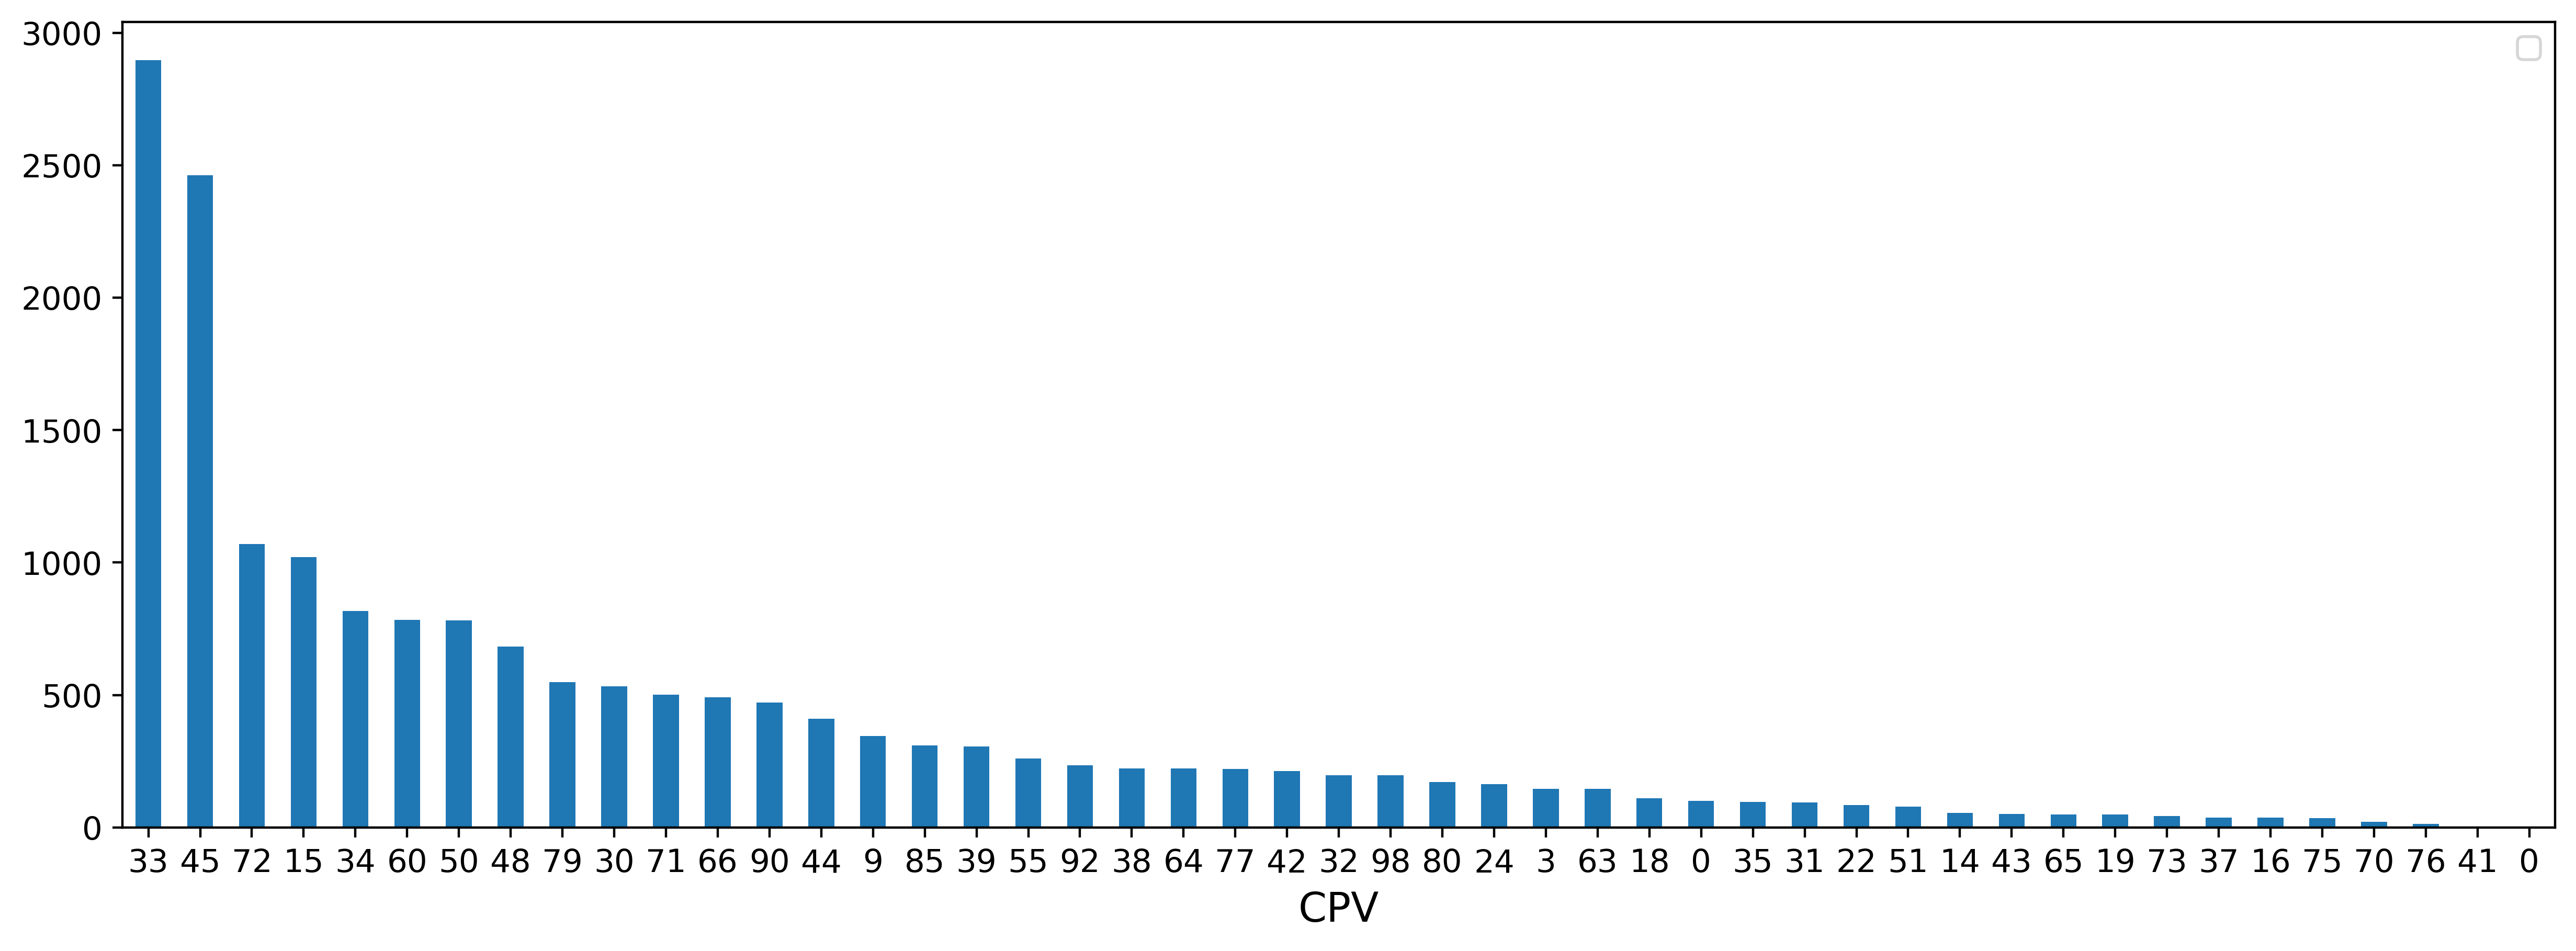
\includegraphics[width=\textwidth]{imagens/r018.png}
	\caption{Grupos com maior número de contratos indiciados}
	\label{}
\end{figure}

\subsection{R019 : Análise do Número de Entidades Concorrentes}

\Lemma{}
	{
	Low number of bidders for item and procuring entity. Number of bidders significantly less than average, based on prior similar contracts (for similar item or procuring entity) 
	}


Para a construção deste indicador, foi necessário construir uma tabela adicional. Para cada uma das 46 divisões de CPV, foi feita uma contagem de todos os contratos, calculado o número total de entidades concorrentes de entre todos os contratos e foram calculados os seguintes indicadores estatísticos : média, desvio-padrão, primeiro-quartil, segundo-quartil, terceiro-quartil, mínimo e máximo. Este procedimento foi feito através de um script \textit{python}, obtendo-se uma tabela do género : 

\begin{table}[H]
	\centering
	\begin{tabular}{|c|c|c|c|c|c|c|c|c|c|}
		\hline
		\textbf{cpv} & \textbf{nec\_t} & \textbf{count} & \textbf{mean} & \textbf{std} & \textbf{min} & \textbf{q1} & \textbf{q2} & \textbf{q3} & \textbf{max} \\ \hline
		98           & 1739            & 586            & 2.968         & 2.251        & 1            & 1           & 2           & 4           & 15           \\ \hline
	\end{tabular}
	\caption{}
\end{table}

sendo que \textbf{cpv} corresponde a cada umas das divisões de CPV, \textit{nec\_t} corresponde ao número total de entidades concorrentes em todos os concursos, \textit{count} é número total de contratos, \textbf{mean}, \textbf{std}, \textbf{min}, \textbf{q1}, \textbf{q2}, \textbf{q3} e \textbf{max} são, respetivamente, o valor médio, o desvio padrão, mínimo, primeiro quartil, segundo quartil, terceiro quartil e máximo para todos os contratos cujos primeiros dois digitos do CPV sejam iguais aos da primeira coluna. 

Com o resultado obtido, foi feita, numa primeira instância, uma representação gráfica dos valores da média, mediana e desvio-padrão, por CPV, a fim de ter uma ideia da dispersão - distância entre a média e o desvio padrão - e simetria da distribuição - distância entre média e mediana - dos preços contratuais.

\begin{figure}[!htbp]
	\centering
	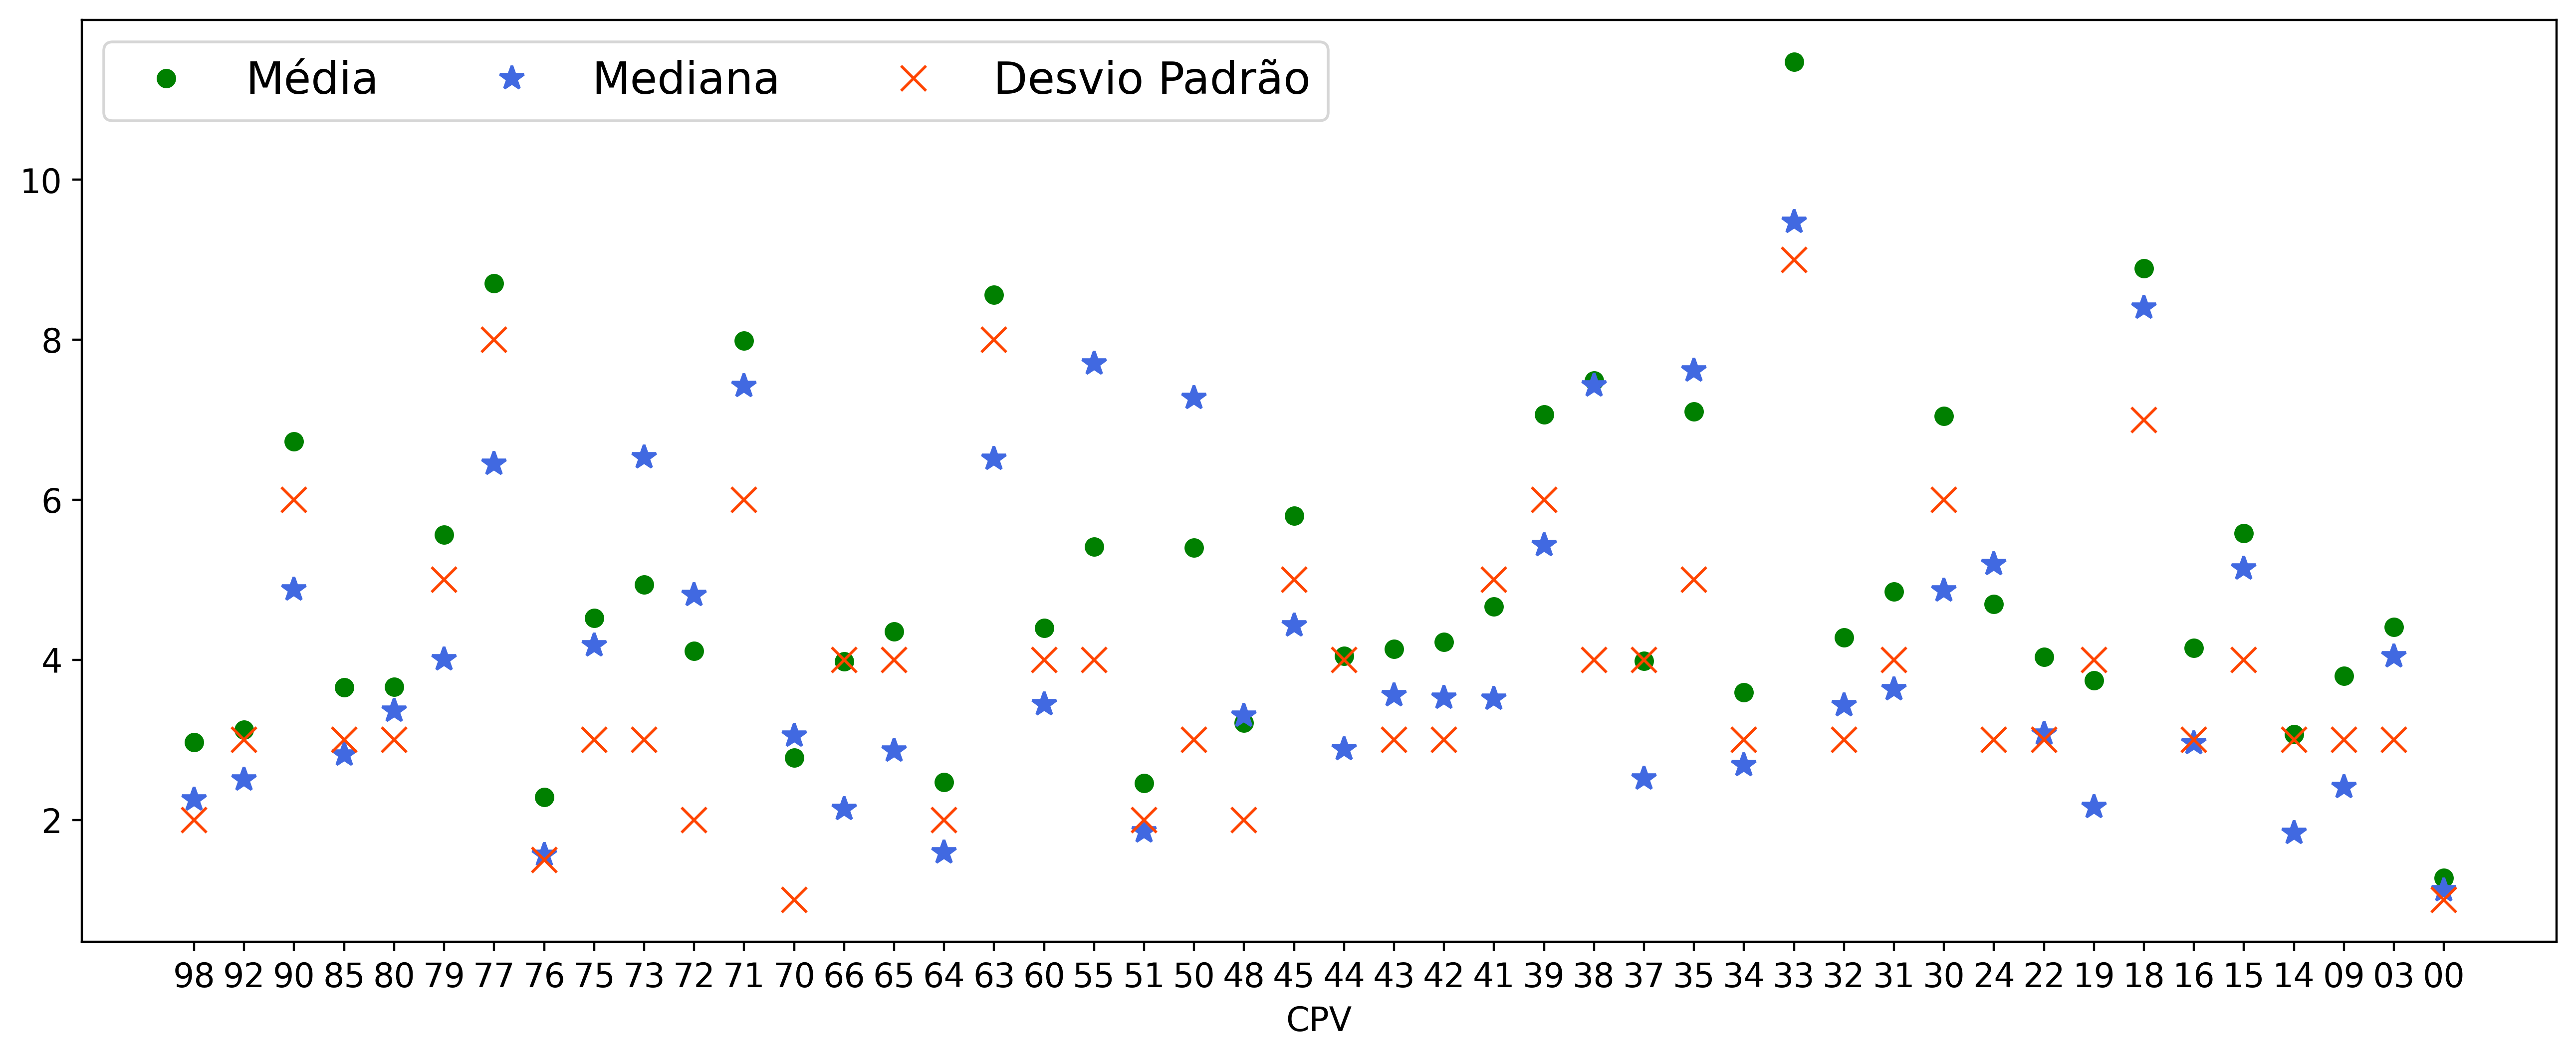
\includegraphics[width=\textwidth]{imagens/mmdp.png}
	\caption{Comparação da Média, Mediana e Desvio Padrão do NEC em CP por CPV}
	\label{}
\end{figure}

Foi, também, feita uma representação gráfica do boxplot para cada umas divisões do CPV. 

\begin{figure}[!htbp]
	\centering
	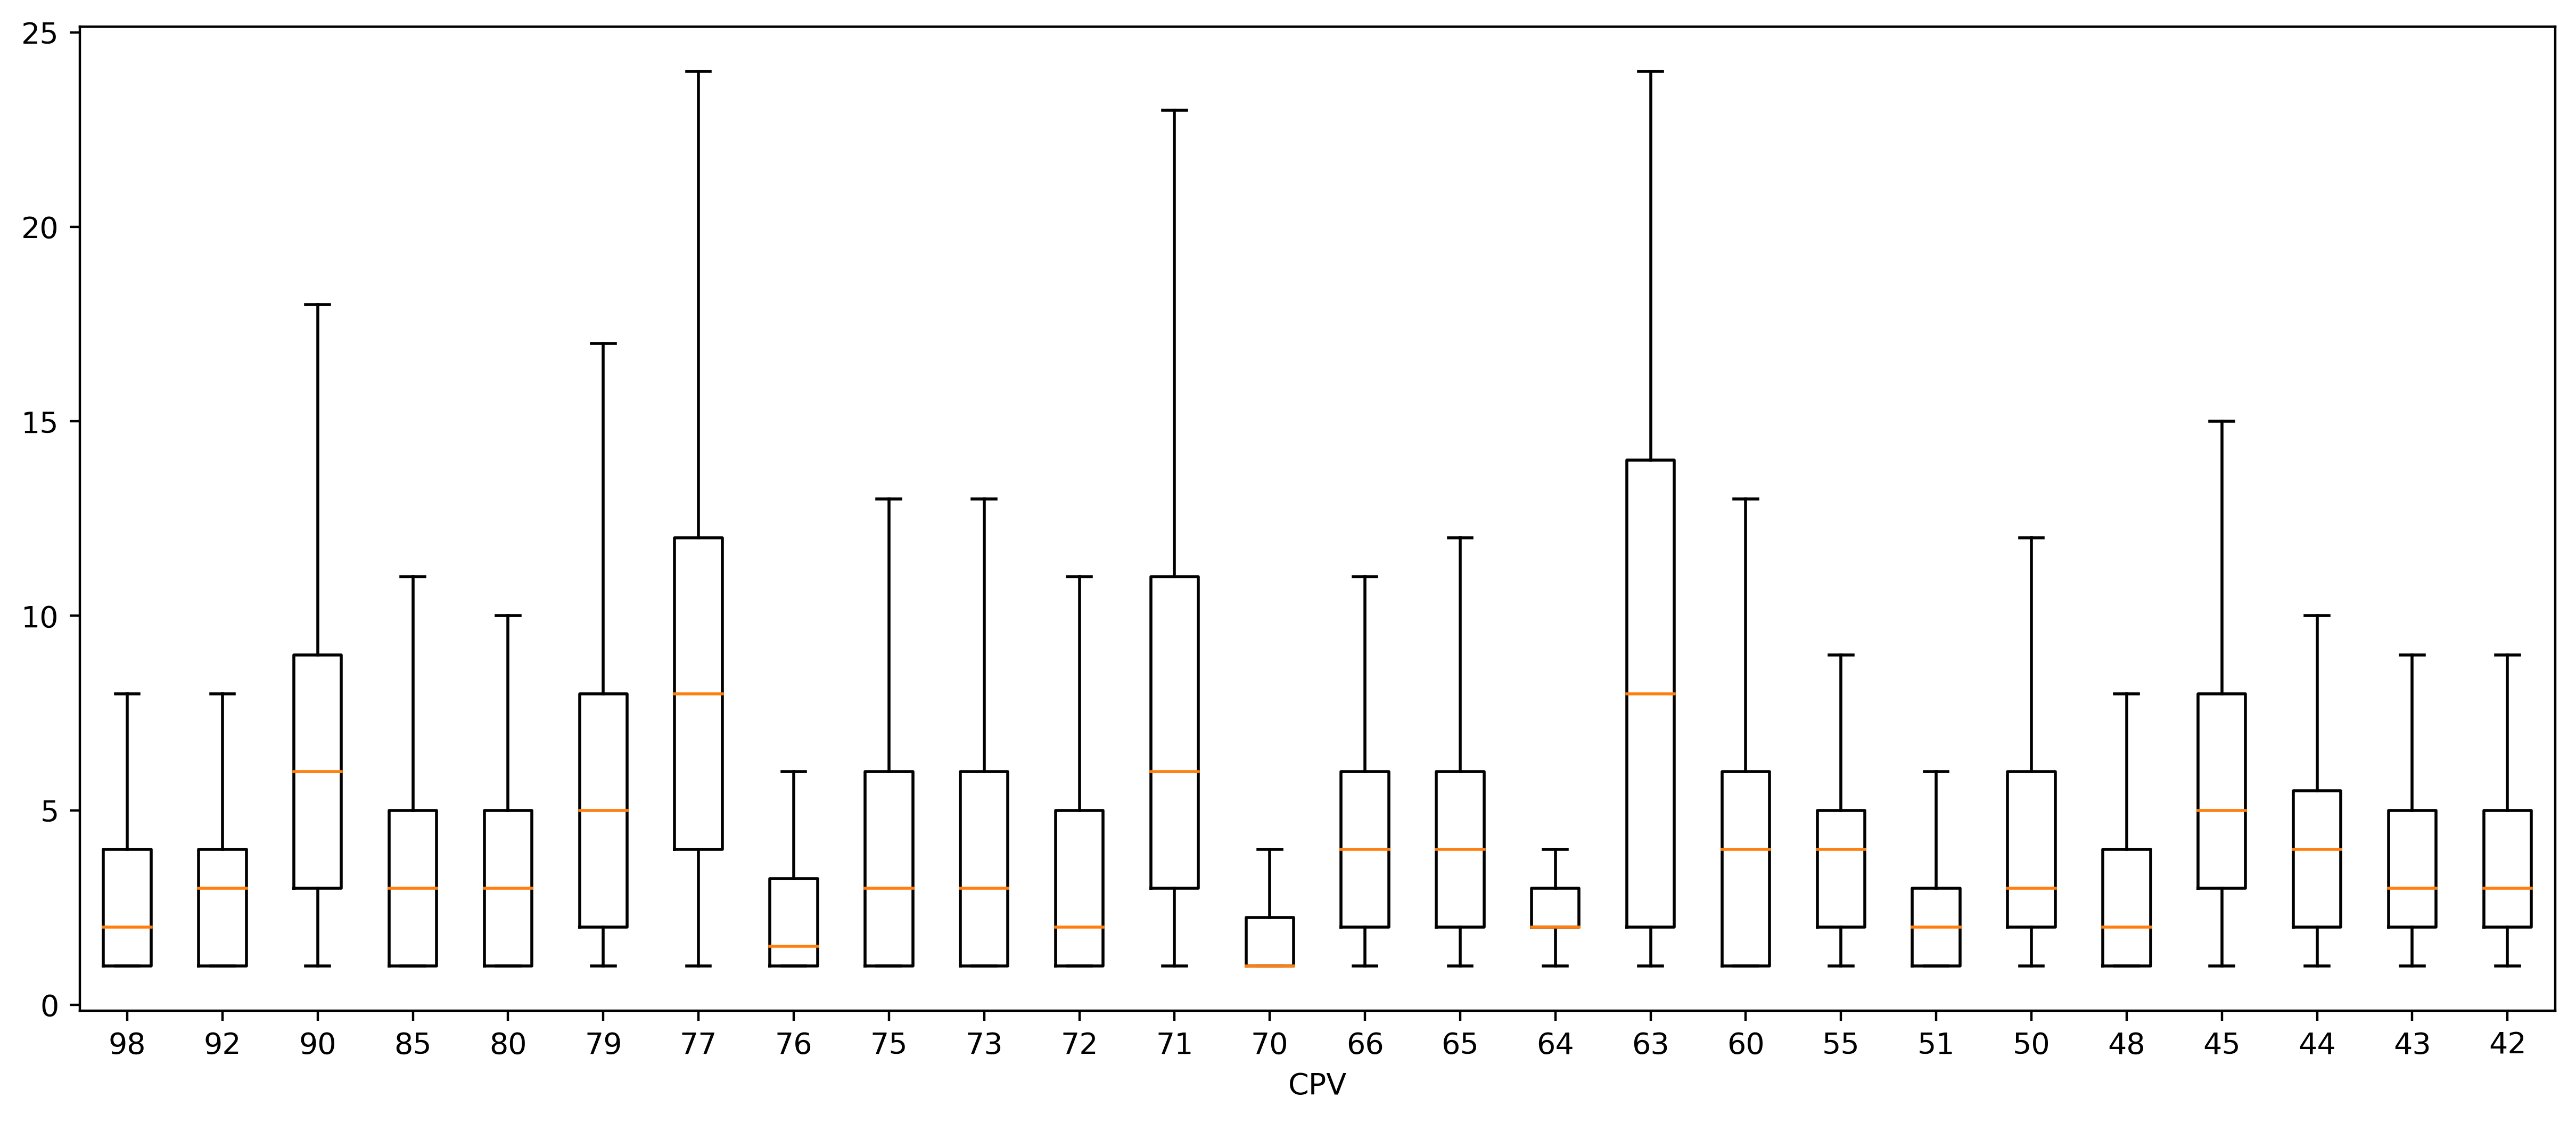
\includegraphics[width=.9\textwidth]{imagens/cpv1.png}
	\caption{Boxplot referente ao número de entidades concorrentes em Concursos Públicos por CPV : I}
	\label{}
\end{figure}


\begin{figure}[h!]
	\centering
	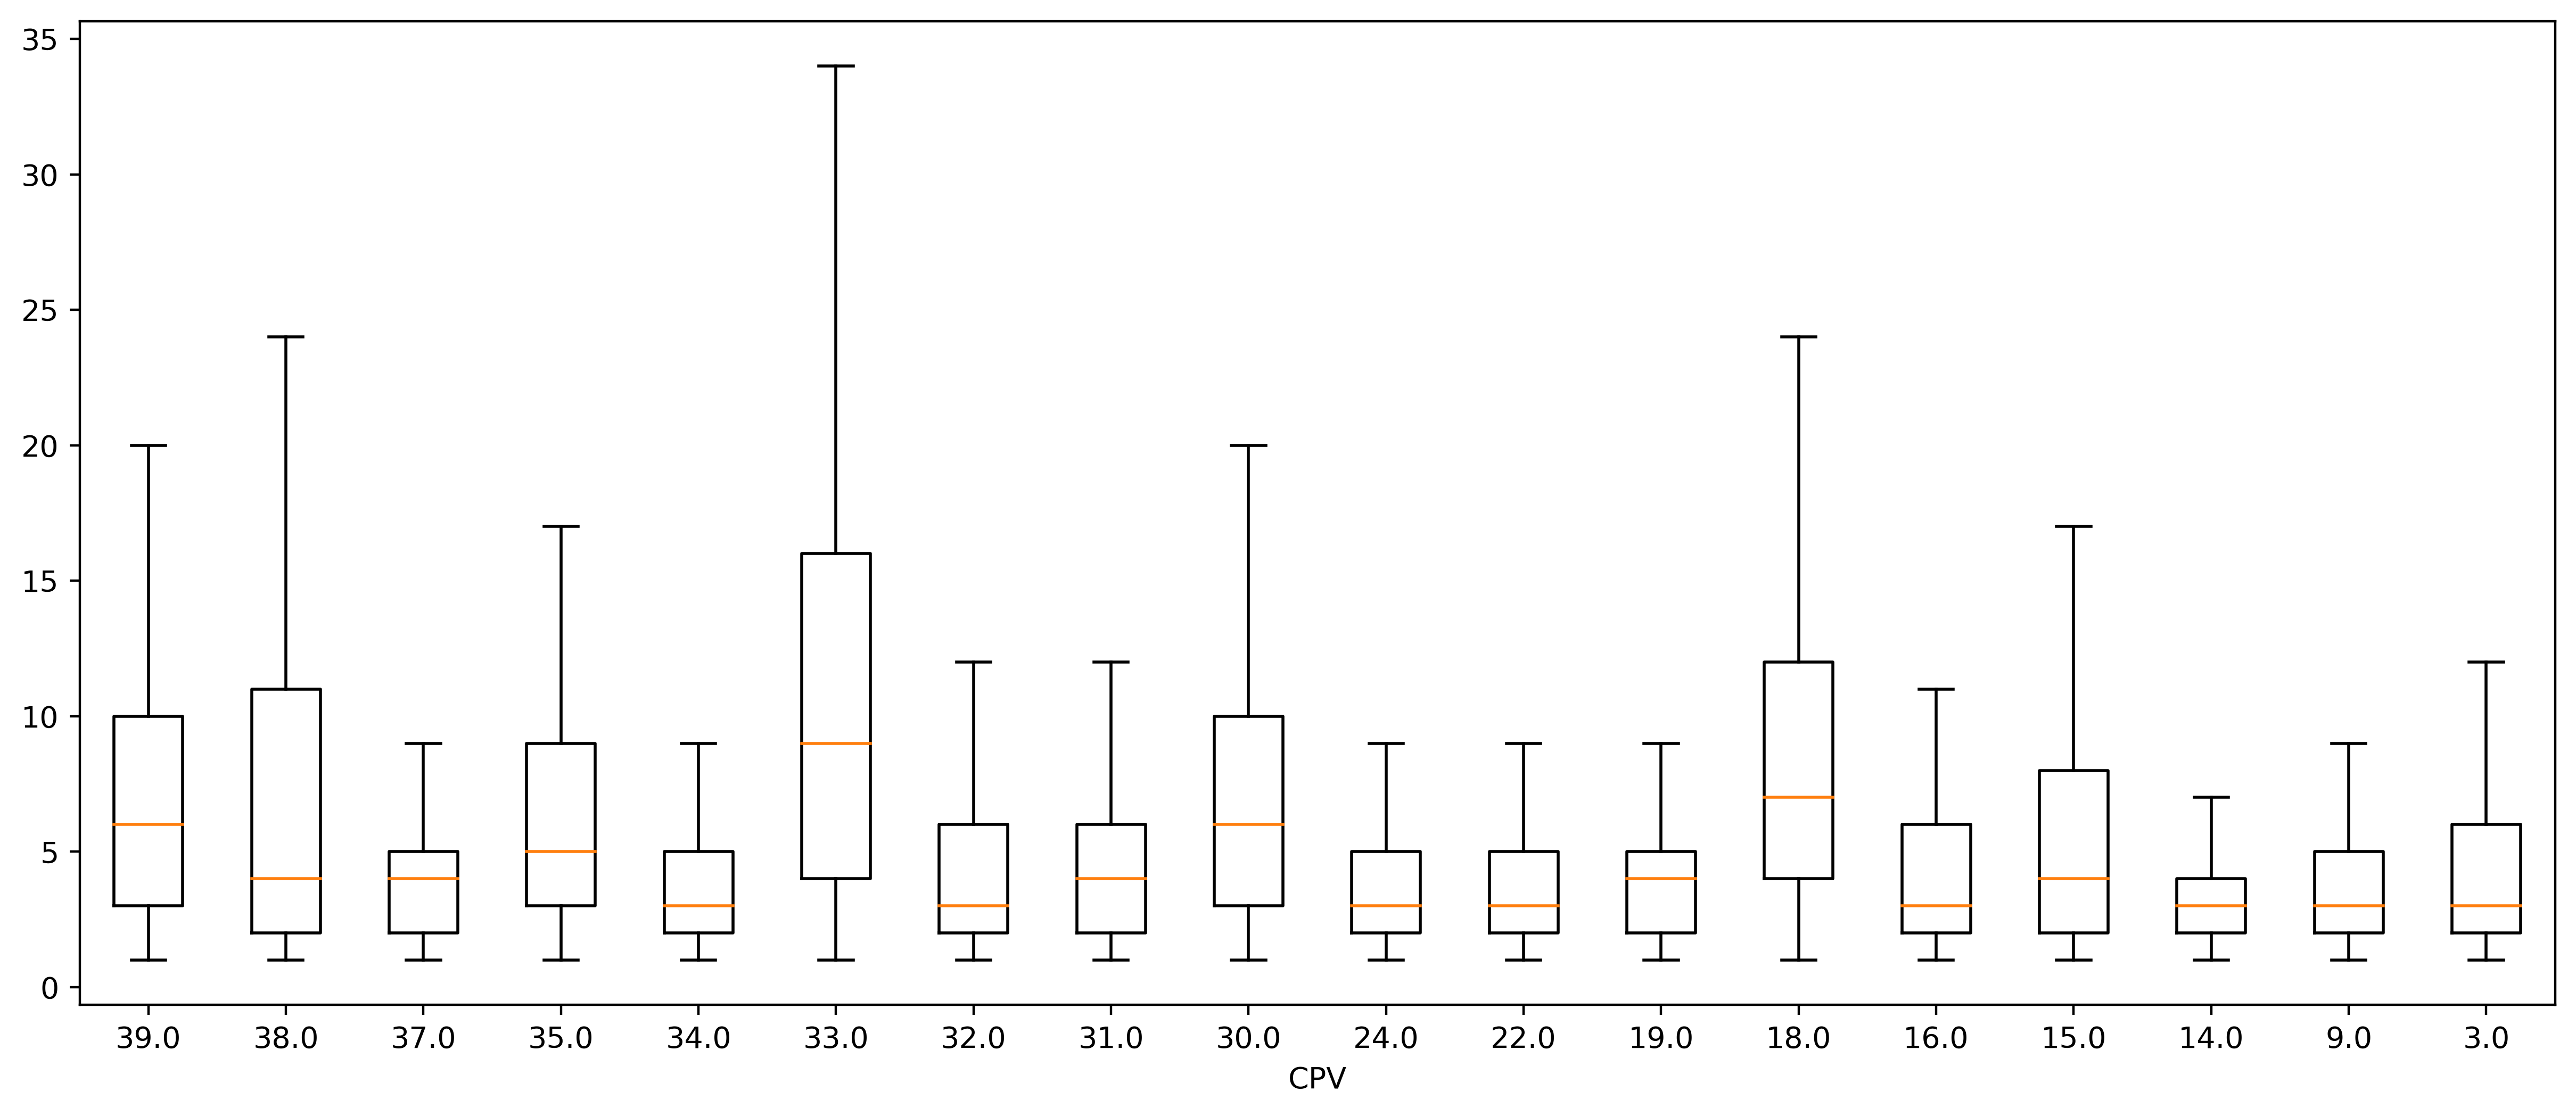
\includegraphics[width=.9\textwidth]{imagens/cpv2.png}
	\caption{Boxplot referente ao número de entidades concorrentes em Concursos Públicos por CPV : II}
	\label{}
\end{figure}


Assim, a fim de selecionarmos os IDs de todos os contratos que respeitem a definição enunciada anteriormente, foi construída a seguinte \textit{query} que retorna todos os contratos cujo número de entidades concorrentes seja inferior à metade do número de entidades concorrentes esperado.  

\begin{lstlisting}[
	language=SQL,
	showspaces=false,
	basicstyle=\ttfamily,
	numbers=left,
	numberstyle=\tiny,
	commentstyle=\color{gray}, frame = single,
	breaklines=true,
	autogobble =true,
	postbreak=\mbox{\textcolor{red}{$\hookrightarrow$}\space},
	]
	SELECT concursospublicos."id"
	FROM concursospublicos 
	JOIN cpv_stat ON concursospublicos."cpv2" = cpv_stat."cpv"
	WHERE concursospublicos."nr_entidadesconcorrentes" < 0.5 * cpv_stat."mean";
\end{lstlisting}

Os resultados obtidos, que podem ser observados na seguinte figura, mostram que existe uma forte predominância dos CPVs começados por 33 e 45, o que pode ser um indicador de que existe um elevado número de contratos com um número \textit{baixo} de entidades concorrentes. 

\begin{figure}[H]
	\centering
	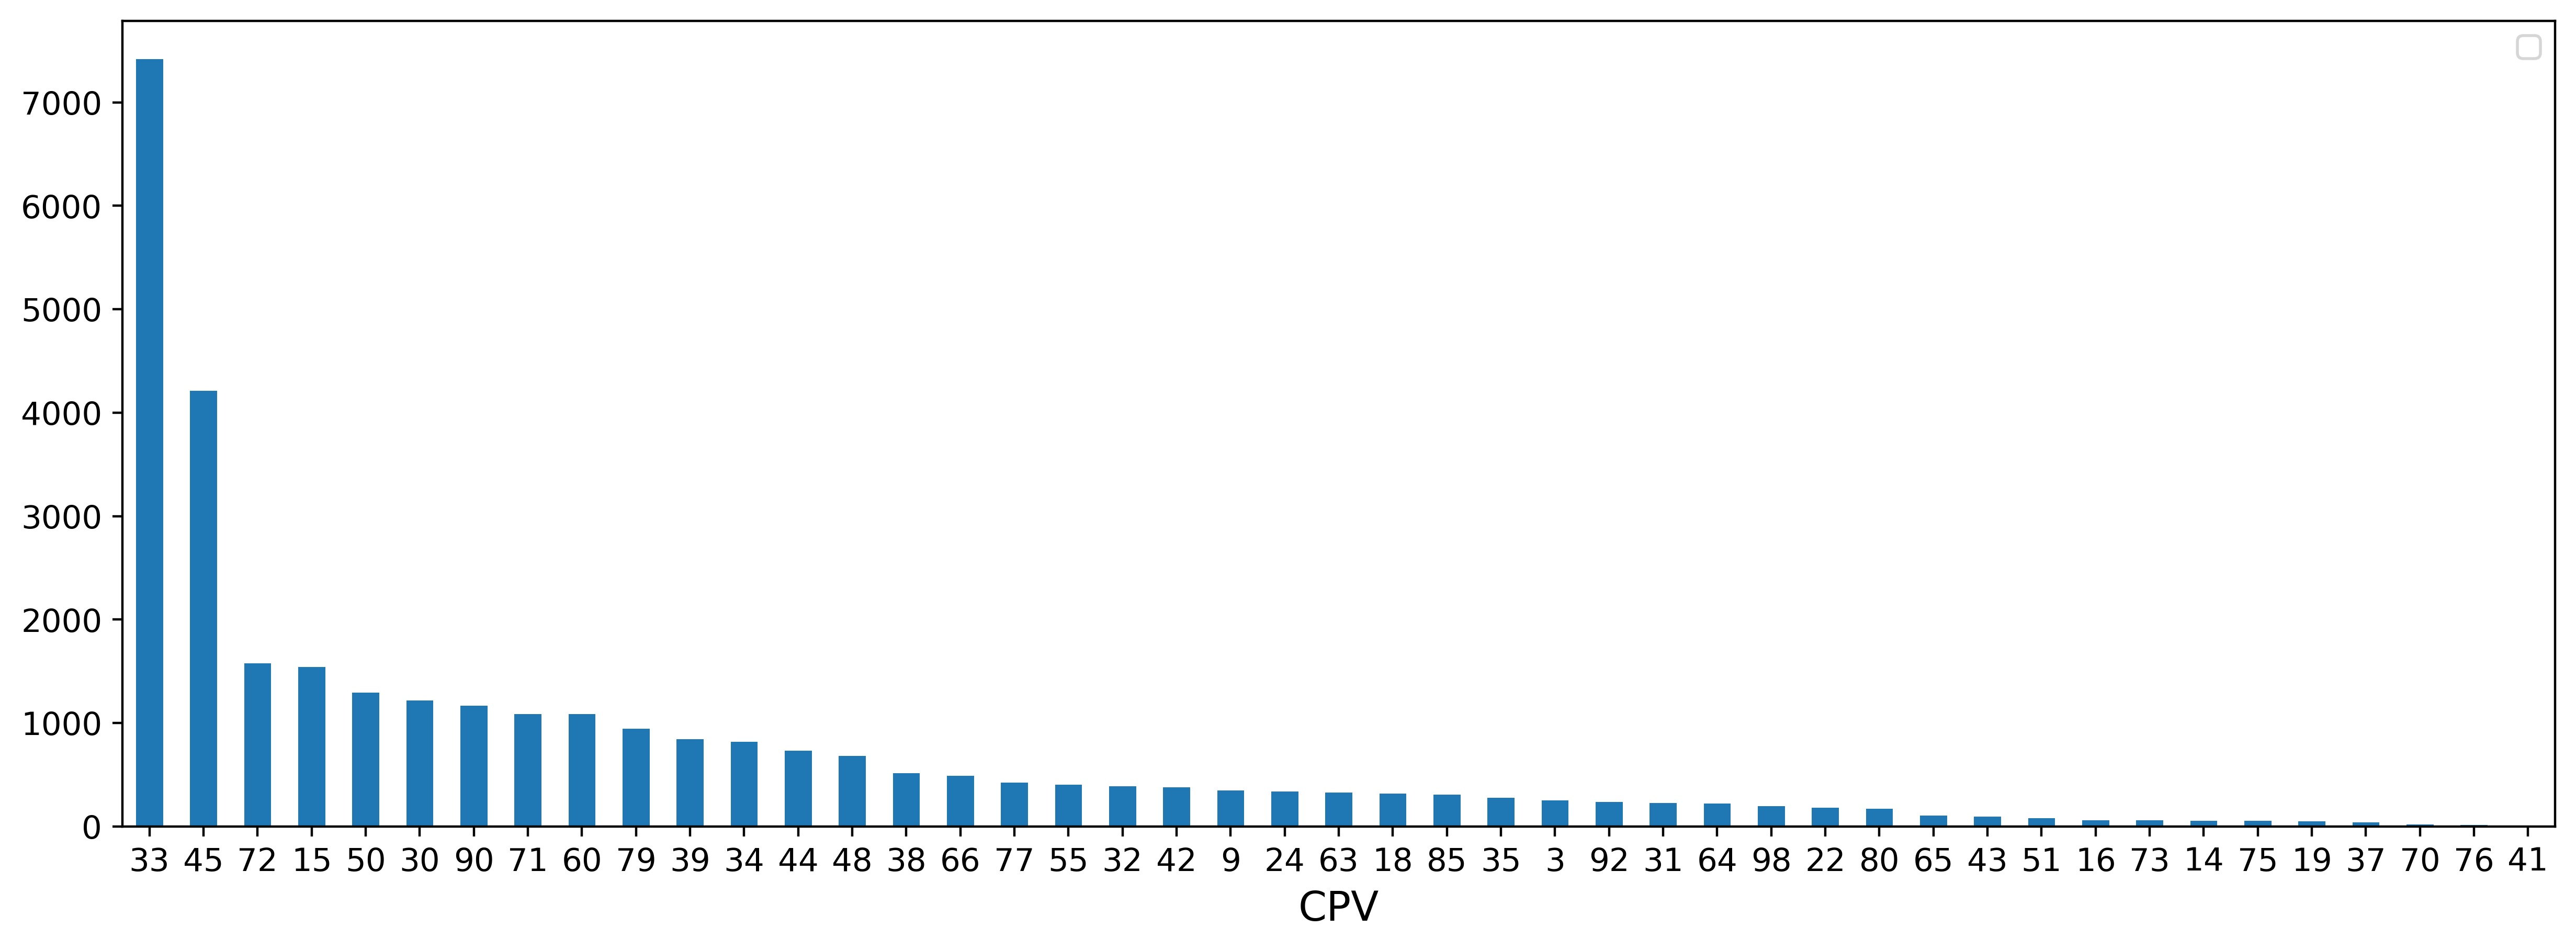
\includegraphics[width=\textwidth]{imagens/r019.png}
	\caption{Grupos com maior número de contratos indiciados}
	\label{}
\end{figure}





\subsection{R031 : Análise da relação entre Preço Base e Preço contratual}

A primeira flag construída tem como objetivo comparar o preço base com o preço contratual.


Numa primeira instância, pegou-se num \textit{subset} de contratos da base de dados em PostgreSQL e guardou-se numa \textit{dataframe} em Python. 
Utilizando a função \textit{cpv}, obtiveram-se os id's dos contratos de um dos tipos de contrato desejados e para um determinado cpv. Numa fase inicial optou-se pelos ids concursos públicos para CPV's começados por 72. 


Para se poder comparar ambos os preços foram desenvolvidas algumas funções auxiliares.
Primeiramente, desenvolveu-se a função \textit{preco\_contratual1} que devolve, a partir do id de um anúncio, o valor do preço contratual desse mesmo anúncio.
A função \textit{preco\_contratual2} faz o mesma coisa mas para um tabela genérica pertencente à base de dados. A função \textit{preco\_contrato3} generaliza a primeira função, pois retorna um conjunto de preços contratuais referentes a um conjunto de ids de anúncios que leva como input. A função \textit{preco\_contratual4} generaliza a função anterior para qualquer tabela. Os precos contratuais são retornados no formato de array.


De seguida, foi feito o mesmo para o preço base. Foi utilizada a mesma abordagem e construíu-se a função \textit{preco\_base3} que retorna os valores dos preços base para um conjunto de id's. 


Assim, foi construída uma primeira versão para esta flag. 

\begin{verbatim}
	def redflag(pbase, pcontr, tol, ids, r, df):
\end{verbatim}

Definiram-se como parâmetros de entrada desta função o conjunto de preços bases - pbase - e preços contratuais - pcontr - associados a um determinado conjunto de ids - ids - que já conseguimos determinar usando as funções criadas anteriormente. É preciso fornecer uma tolerância - tol - que vai definir a diferença máxima permitida entre o preço base e o contratual e um racio máximo permitido entre o preco base e contratual. 


O objetivo desta flag é identificar todos os contratos cujo preço contratual pertença a um intervalo em torno do preço base, definido pelo parâmetro \textit{tol}.

\begin{figure}[H]
	\centering
	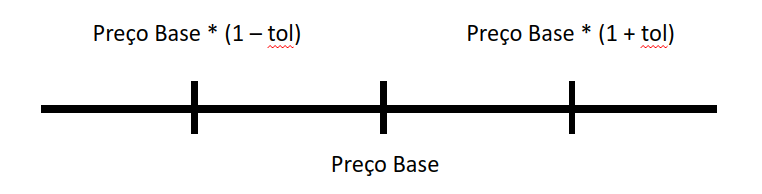
\includegraphics[width=0.7\textwidth]{imagens/pbasecontr.png}
	\caption{}
	\label{}
\end{figure}


%O preço base é conhecido à priori, por isso esta flag não tem muito valor por si só. Quando for acoplada com outras flags pode sugerir um comportamento suspeito. Também é preciso ter em conta como é que o preço base é calculado. Se o preço base for calculado por excesso e o preço contratual for próximo do preço base, pode haver corrupção tanto por parte da entidade adjudicante como da adjudicatária. 

Contudo, ao longo da construção desta flag verificou-se a existência de casos em que o preço base é significativamente superior ao preço contratual, chegando a atingir uma ordem de grandeza de $\approx 10^2$. Isto deve-se a dois fatores : o preço base definido é demasiado elevado comparativamente ao preço contratual ou o preço base diz respeito a casos em que a adjudicação de um determinado serviço/obra é feita por lotes.

\begin{table}[H]
	\centering
	\begin{tabular}{|c|c|c|c|c|}
		\hline
		\multicolumn{1}{|l|}{\textbf{Número de Anúncio}} & \multicolumn{1}{l|}{\textbf{ID}} & \multicolumn{1}{l|}{\textbf{Lote}} & \multicolumn{1}{l|}{\textbf{Preço Base}} & \multicolumn{1}{l|}{\textbf{Preço Contratual}}          \\ \hline
		& 10471090                         & 1                                  &                                          & \cellcolor[HTML]{F2FCFE}{\color[HTML]{555555} 77454.72} \\ \cline{2-3} \cline{5-5} 
		& 10471049                         & 2                                  &                                          & \cellcolor[HTML]{F2FCFE}{\color[HTML]{555555} 85365.84} \\ \cline{2-3} \cline{5-5} 
		\multirow{-3}{*}{11171/2023}                     & 10470972                         & 3                                  & \multirow{-3}{*}{373860.48}              & \cellcolor[HTML]{F2FCFE}{\color[HTML]{555555} 89886.72} \\ \hline
	\end{tabular}
	\caption{Exemplo de contrato adjudicado por lotes}
\end{table}


Tendo em conta que na base de dados não é disponibilizado o preço base para cada lote, foi utilizada a seguinte abordagem. É de salientar que no caso de adjudicação por lotes, o número de anúncio é igual para cada um dos lotes, mas cada lote tem um id diferente. 

Sempre que o rácio $\text{preçobase} / \text{preçocontratual}$, para um certo contrato, é superior a determinado limite, o respetivo id é guardado. A partir do id do contrato obtém-se o número do anúncio e, para todos os contratos com o mesmo número de anúncio, são somados os preços contratuais e o resultado final é comparado com o preço base. 

Por fim, o resultado final é um conjunto de id's na forma de tuplo que respeita as condições anteriormente mencionadas.




%\section{Análise dos Concursos Públicos}
%
%Aqui só foram usadas funções ja definidas. Criaram-se variáveis que guardam o valor do preço base e contratual dos concursos. Deu-se isso como input à funcao \textit{redflag}, além dos outros que são definidos por mim, e obtiveram-se as redflags. Representou-se um barplot dos precos contratuais em cima dos preços base para verificar a diferença entre os mesmos. 


%\section{Análise dos Ajustes Diretos em Regime Geral}
%
%Aqui, novamente, foram utilizadas as funções já criadas anteriormente para obter uma dataframe com os contratos referentes a ajustes diretos e os ids associados. Foi feito um sumário estatístico dos valores dos preços contratuais e um histograma e um boxplot. Mas como tem outliers, vê-se mal. 
%Ordenei os ajustes diretos por fundamentação. Não nenhum campo vazio. 
%Com isto tudo ja se podem calcular as flags usando a função \textit{redflag2}. 
%É interessante saber qual a proporção de atividades suspeitas por entidade adjudicante e entidade adjudicatária. Para isso, calculou-se primeiro o número de contratos suspeitos e respetiva percentagem. 
%Para conseguir analisar foi preciso separar as colunas das entidades adjudicantes e adjudicatárias - que estavam no formato Entidade(NIF)(URL) - em três colunas distintas para cada uma das duas entidades. Isto é necessário para filtrar os contratos pelo NIF porque diferentes entidades podem ter o mesmo NIF. 
%Depois disso, ordenou-se por ordem decrescente de ajustes diretos realizados os NIFS das empresas. Uma das listas ordenadas só para as entidades adjudicantes, outra para as entidades adjudicatárias. 
%Para esta analise foi necessário criar duas funções que retornem os ids dos ajustes diretos a partir do NIF da empresa. Queremos todos os ajustes diretos celebrados para um determinada entidade a partir do seu NIF. Isso foi feito a partir das funções \textit{e\_adjudicante} e \textit{e\_adjudicataria}. 
%De seguida, foi então calculado para cada NIF o número de ajustes diretos realizados usando uma das funções anteriores e os respetivos ID's. Para cada NIF, foi comparado cada um dos nos id's com a lsita de id's dado pela função \textit{redflags2} e feito o rácio para ver a percentagem de contratos suspeitos. 
%Agora seria interessante verificar se existem, dentro destas empresas, subgrupos entre entidades adjudicantes e adjudicatárias. 



\subsection{RF2 : Comparação entre Preço Contratual e Preço Total Efetivo}

Existem situações em que o valor contratual celebrado é alterado após celebração do contrato. Estes valores são guardados na coluna referefente ao Preço Total Efetivo. Nesses casos, é simples verificar quais são os contratos em que ocorre esta situação através de uma \textit{query}: 


\begin{lstlisting}[
	language=SQL,
	showspaces=false,
	basicstyle=\ttfamily,
	numbers=left,
	numberstyle=\tiny,
	commentstyle=\color{gray},	frame=single,
	breaklines=true,
	autogobble = true,
	postbreak=\mbox{\textcolor{red}{$\hookrightarrow$}\space},
	]
	SELECT id
	FROM concursospublicos 
	WHERE preco_total_efetivo > 0 AND ABS(preco_total_efetivo - preco_contratual) > 0;
\end{lstlisting}


\begin{figure}[H]
	\centering
	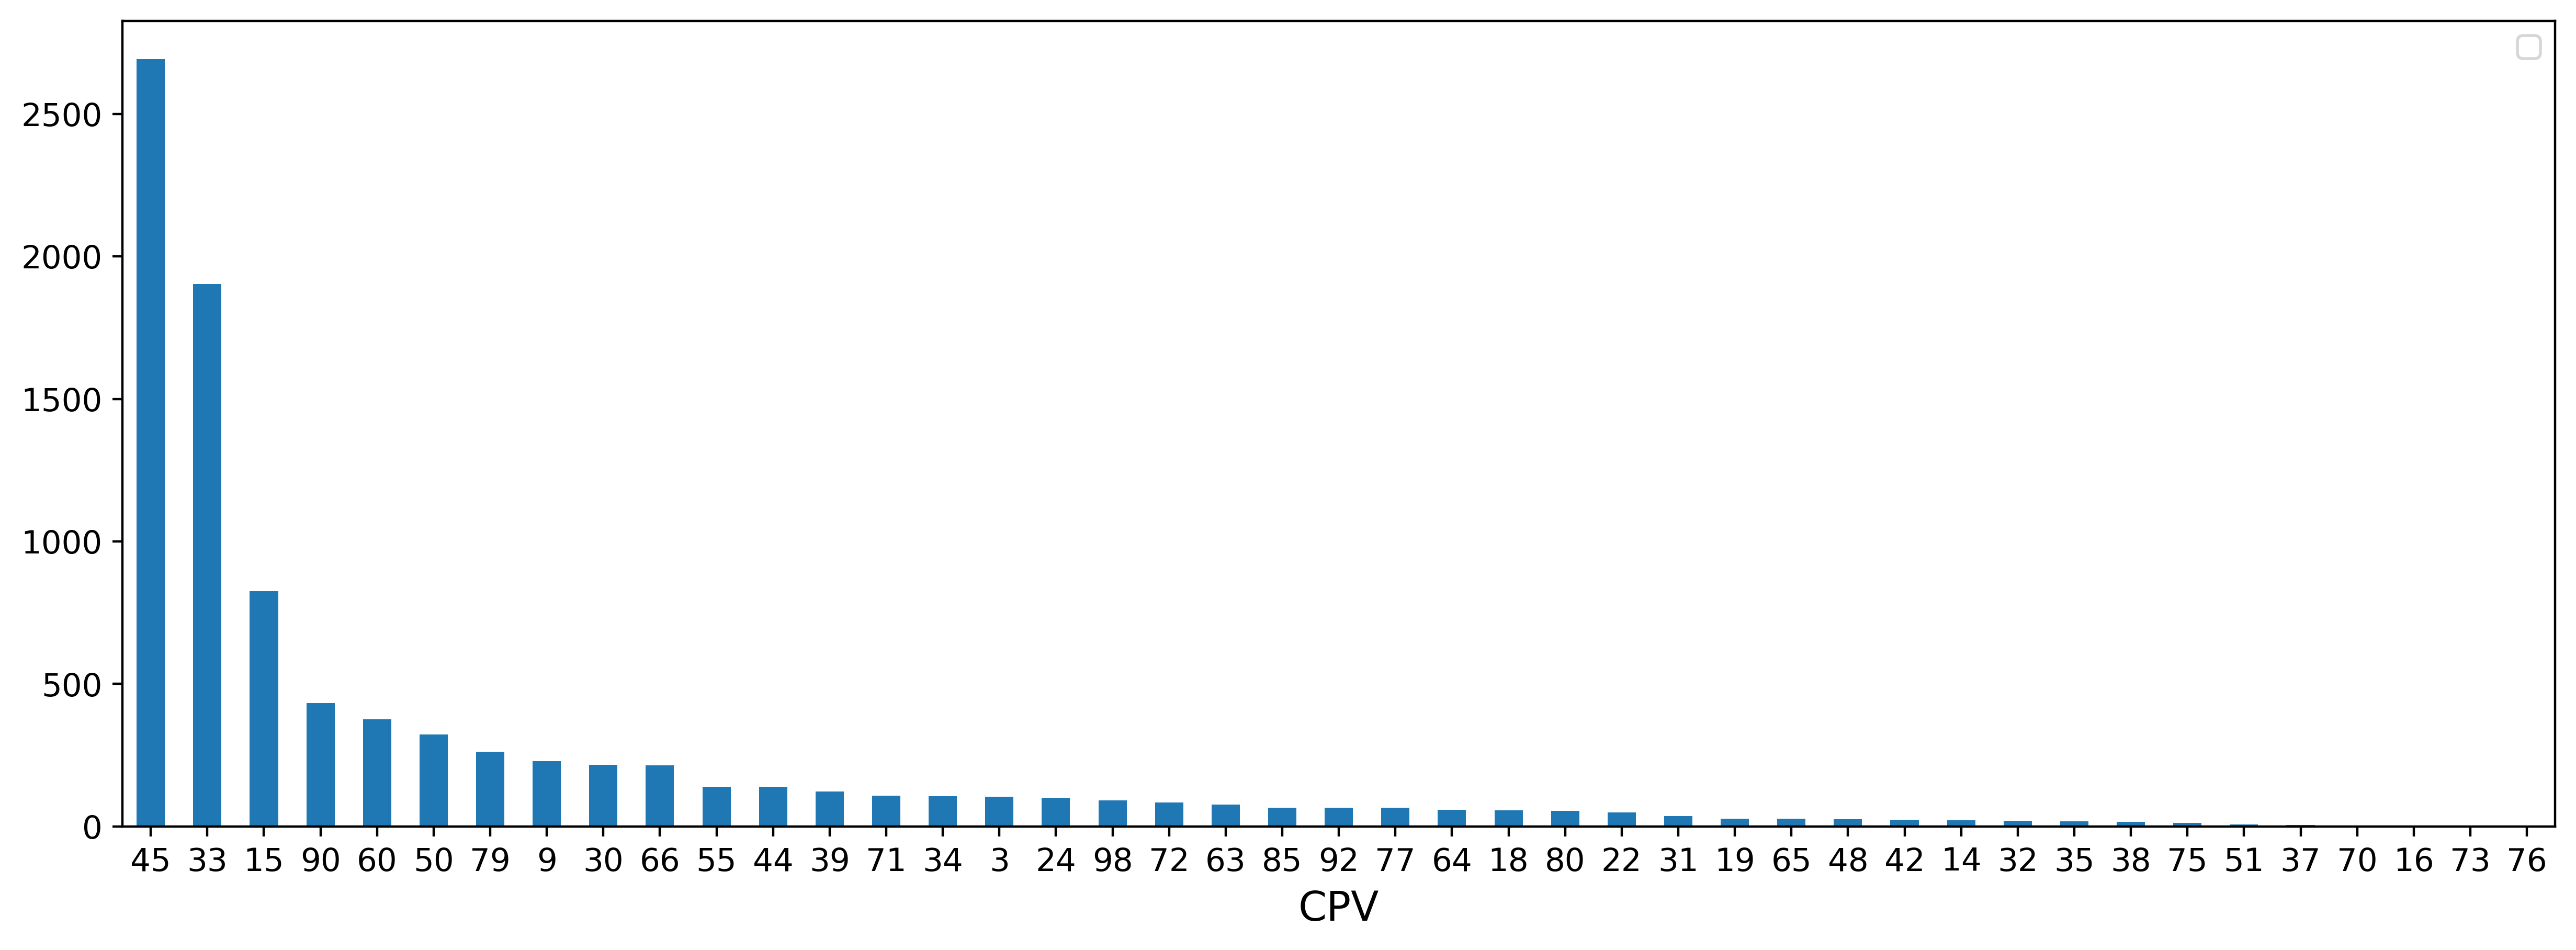
\includegraphics[width=\textwidth]{imagens/r059.png}
	\caption{Grupos com maior número de contratos indiciados}
	\label{}
\end{figure}



\subsection{RF3 : Análise da data de publicação do anúncio}

Adicionalmente, foi feita uma análise do dia de publicação do anúncio em Diário da Reopública. O objetivo deste indicador é verificar se existem anúncios publicados em dias não convencionais - feriados nacionais - na tentativa de os fazer passar despercebidos.


\begin{figure}[H]
	\centering
	\begin{minipage}{.6\linewidth}
		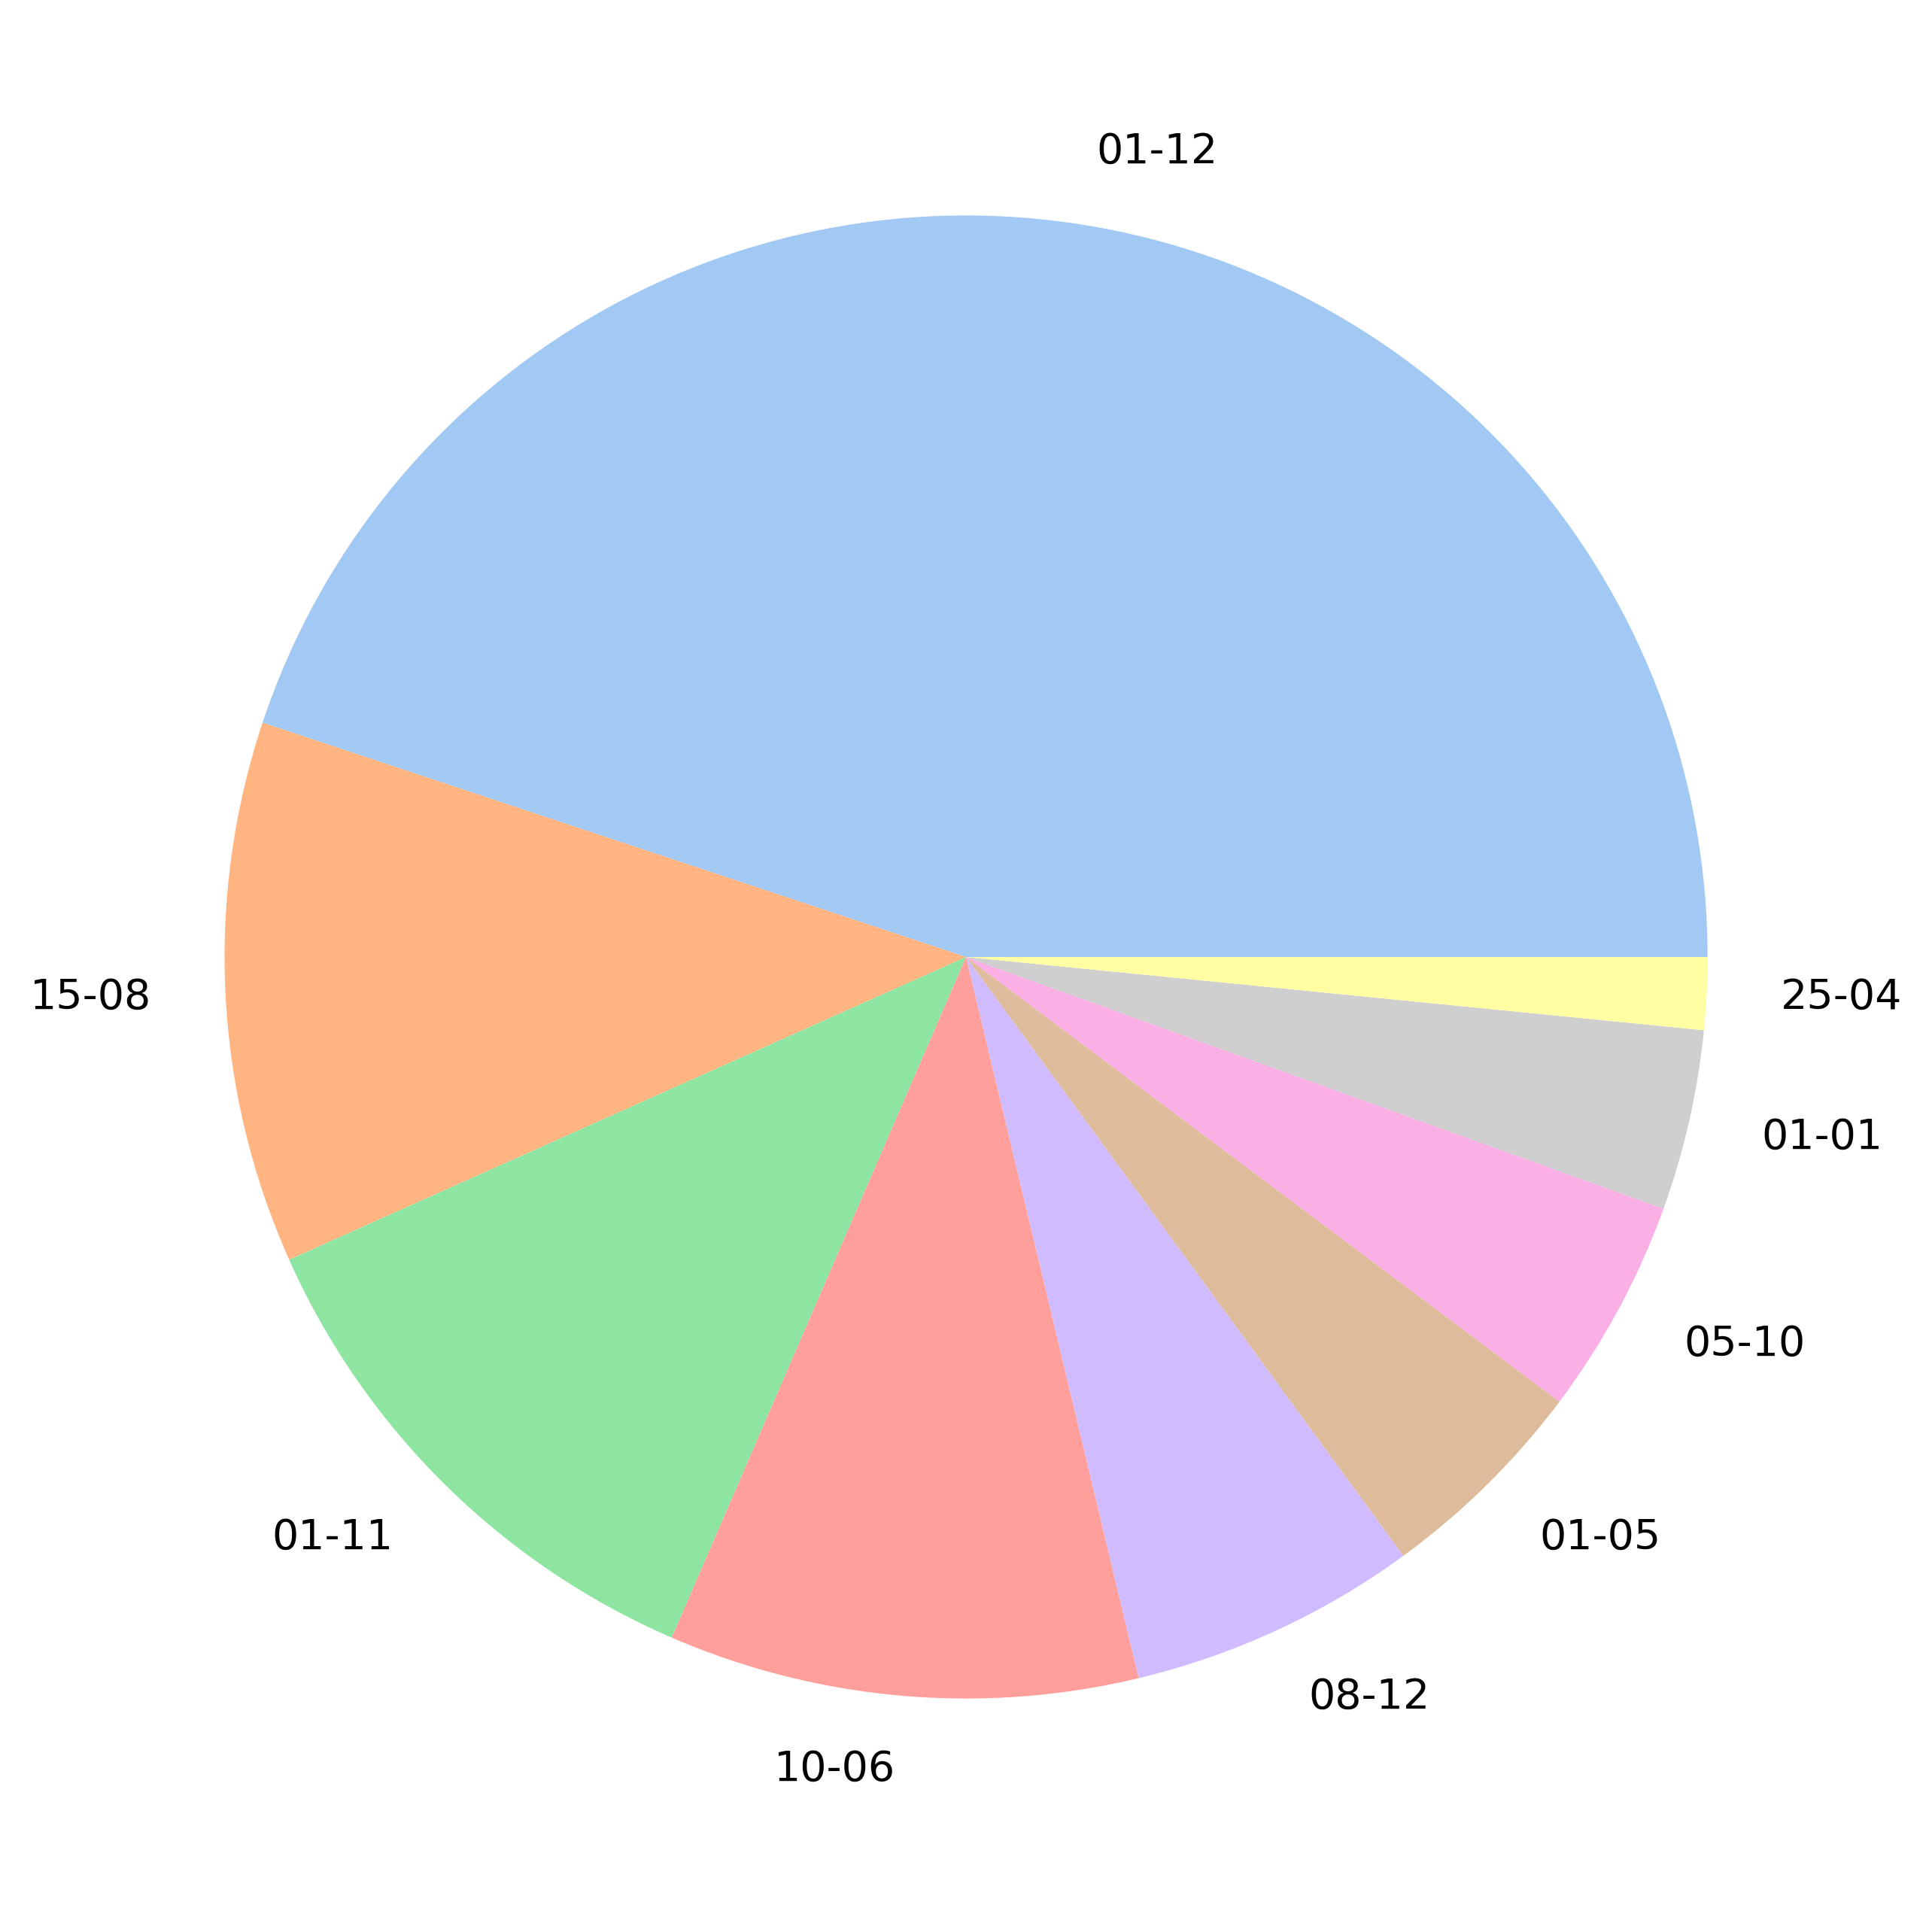
\includegraphics[width=\textwidth]{imagens/pieplot.png}
		\caption{Pieplot do número de ocorrências para anúncios publicados em feriado}
		
	\end{minipage}
	\hfill
	\begin{minipage}{.38\linewidth}
		
			\begin{tabular}{|c|c|}
				\hline
				\textbf{Feriado} & \textbf{Ocorrências} \\ \hline
				01-12            & 57                   \\ \hline
				15-08            & 15                   \\ \hline
				01-11            & 15                   \\ \hline
				10-06            & 13                   \\ \hline
				08-12            & 8                    \\ \hline
				01-05            & 6                    \\ \hline
				05-10            & 6                    \\ \hline
				01-01            & 5                    \\ \hline
				25-04            & 2                    \\ \hline
			\end{tabular}
			\caption{Número de ocorrências para cada feriado}
	\end{minipage}
\end{figure}





